\documentclass{article}
\usepackage[utf8]{inputenc}
\usepackage{graphicx}
\usepackage{here}
\usepackage{amsmath}

\title{Notes de cours\\TC1 : Apprentissage}
\author{Adrien Pavao}
\date{September 2017}

\begin{document}

\maketitle

\tableofcontents

\section{Rappel}

\subsection{Espérance}

Soit une variable aléatoire X, l'espérance : $E[X] = \sum_{x \in A_x} P(X = x) \times x$

Exemple si X suit une loi $N(\mu, \sigma)$ 

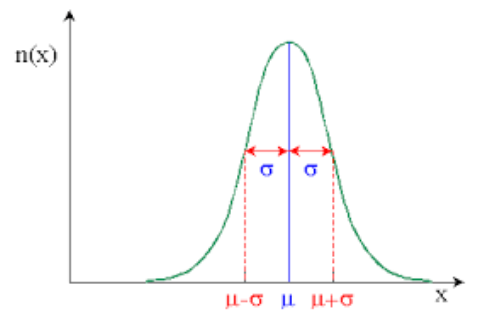
\includegraphics[scale=0.4]{loinormale.png}

$E[X] = \mu$

Pour une variable discrète, ce n'est pas toujours pertinent. De même pour des variables qualitatives plutôt que quantitatives. On préfère donc définir une fonction de cette variable alétoire, et l'espérance de cette fonction. Cela permet de "donner du sens". Ainsi :

\[ E[f(X)] = \sum_x P(X = x) \times f(x) \]

X dépend de la distribution tirée sur la variable aléatoire. On note $X \sim P$.

\section{Inférence Bayesienne}

On considère différents niveaux d'inférence.

\subsection{Niveau 1 : Classification Bayesienne}

\begin{itemize}
\item Y : La classe à prédire (catégorielle)
\item $\vec{X}$ : Vecteur aléatoire, \( \vec{X} 
\begin{pmatrix} 
      x_1\\ 
      ...\\
      x_2 
\end{pmatrix} \)

\end{itemize}

On cherche à choisir y de façon à maximiser : 

\[ P(Y=y | \vec{X} = \vec{x}) = \frac{P(\vec{X} = \vec{x} | Y=y)P(Y=y)}{P(\vec{X} = \vec{x})} \]

Dans cette formule, on remarque des termes particuliers : 

\begin{itemize}

\item La \textbf{vraisemblance} : $P(\vec{X} = \vec{x} | Y = y)$.
\item L'\textbf{a priori} : $P(Y = y)$.
\item L'\textbf{évidence} : $P(\vec{X} = \vec{x})$.

\end{itemize}

La vraisemblance et l'a priori sont à estimer. On estime une ditribution sur X pour chaque classe y.
On peut donc faire l'hypothèse naïve suivante : 

\[ P(\vec{X}=\vec{x} | Y=y) = \Pi_{i=1}^{d} P(\vec{X}_i = \vec{x}_i | Y = y) \]

\subsubsection*{Estimer les paramètres}

Cas Bernouilli : $\Theta_{iy} = \frac{n(1, i, y)}{N(i, y)}$

$ n(1, i, y) =$ nombre de fois où $\vec{X}_i = 1$ dans la classe y.

Si $n(1, i, y) = 0$ alors $\Theta_{iy} = 0$

Donc $P(\vec{X} = \vec{x} | Y = y) = 0$, ce qui est mauvais. On estime $\Theta$ sur les données et on vient à la conclusion qu'un evenement est impossible sous pretexte qu'on ne l'a jamais observé. Il faut éviter ce problème.

Ce type d'estimation est appelée une estimation \textbf{MLE : Maximum Likelihood Estimate}. Il s'agit de l'interprétation \textbf{fréquentiste} des données.

Autrement dit, on cherche les paramètres $\Theta_{iy}$ qui maximisent $P(D | \Theta_{iy})$. (D la réalisation des données ..)

\subsection{Niveau 2 : Inférence Bayesienne des paramètres}

On cherche $P(X_i | Y) \rightarrow P(X_i | Y_i \Theta_{iy})$. L'apprentissage revient à l'estimation d'une distribution sur les paramètres.

Estimer $ P(\Theta_{iy} | D) $.

\[ P(\Theta_{iy} | D) = \frac{P(D | \Theta_{iy})P(\Theta_{iy})}{P(D)} \]

\subsubsection{A priori sur les paramètres}

Cas Bernouilli : $\Theta_{iy} \in [0, 1]$, continu. Donc $P(\Theta_{iy})$ \_ une loi continue de support $[0, 1]$.
Le choix : Loi Beta.

\[ P(\Theta_{iy}; \alpha_0, \alpha_1) = \frac{\Gamma (\alpha_0 + \alpha_1)}{\Gamma (\alpha_0) \Gamma (\alpha_1)} \Theta_{iy}^{\alpha_1 - 1} (1 - \Theta_{iy})^{\alpha_0 - 1} \]

(Dénominateur et game $\rightarrow$ Normalisation)

$\alpha_0$ et $\alpha_1$ sont les paramètres de la loi Beta. On a $\alpha_0, \alpha_1 > 0, \in R$ (R reel, D majuscule ...)

\begin{itemize}
\item \textbf{Fonction de densité symétrique : }

$\alpha_0 = \alpha_1$ et $\alpha_0, \alpha_1 > 1$.

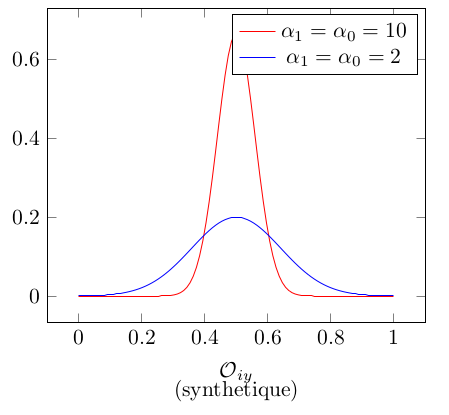
\includegraphics[scale=0.4]{schema1.png}

\item \textbf{A priori non-informatif : }

$\alpha_0 = \alpha_1 = 1$.

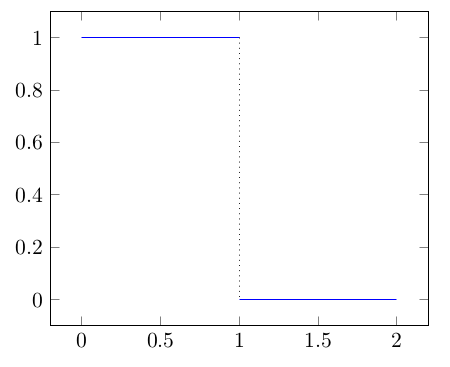
\includegraphics[scale=0.4]{schema2.png}

\item \textbf{A priori parcimonieux (sparse) : }

$\alpha_0, \alpha_1 < 1$

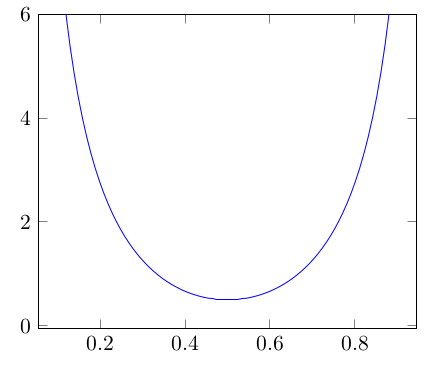
\includegraphics[scale=0.4]{schema3.png}

\end{itemize}

\subsubsection{A posteriori sur les paramètres}

\[ P(\Theta_{iy} | D) \propto P(D | \Theta_{iy}) P(\Theta_{iy}; \alpha_1, \alpha_0) \] (vraimsemblance et a priori).
\[ P(\Theta_{iy} | D) \propto \Theta_{iy}^{N_1 + \alpha_1 - 1} (1 - \Theta_{iy})^{N_0 + \alpha_0 - 1} \]

$\propto$ signifie "proportionnel à".

\begin{itemize}
\item $N_0$ : Nombre de $x_i$ à 0 dans D.
\item $N_1$ : Nombre de $x_i$ à 1 dans D.
\end{itemize}

La loi a posteriori est comme la loi a priori, une loi Beta. La loi Beta est l'a priori \textbf{conjugué} de Bernouilli (conjugated prior).

\subsubsection{Retour à la classification}

\begin{enumerate}

\item \textbf{Maximum a Posteriori des Paramètres (MAP)}

$ \Theta_{iy} = argmax P(\Theta_{iy} | D) $ ( chapeau sur le theta ! )
$ \Theta_{iy} = \frac{N_1 + \alpha_1 - 1}{N_1 + N_0 + \alpha_1 + \alpha_0 - 2} $

$\alpha_1$ et $\alpha_0$ agissent comme des "pseudo-comptes". Lissage (smoothing) de distibution.
$\Theta_{iy} != 0$
Si $N_1, N_0 >> \alpha_1, \alpha_0$ alors l'a priori est négligeable.

La régularisation permet d'éviter le sur-apprentissage.

\item \textbf{Loi prédictive (inférence Bayesienne 3)}

$P(X_i = x_i | Y = y; \Theta_{iy})$ avec $\Theta_{iy}$ estimés à partir des données (MAP).

Le paramètre n'existe pas et ne doit donc pas apparaitre dans la prédiction. La vraie prédiction :

$P(X_i = x_i | D) = integrale01 P(X_i = x_i; \Theta_{iy} | D) d \Theta_{iy}$, en marginalisant les paramètres.

$P(X_i; \Theta_{iy} | D) = P(X_i | \Theta_{iy}; D) P(\Theta_{iy} | D)$ (vraisemblance et a priori).

$ P(X_i = x_i | D) = \frac{N_1 + \alpha_1}{N_1 + N_0 + \alpha_1 + \alpha_0}$, $\forall \alpha_1$ et $\alpha_0 > 0$.

\end{enumerate}

\section{Modèles de mélange (G.M.M.)}

\subsection{Introduction}

Un large champ d'applications :

\begin{itemize}

\item \textbf{Clustering :} Apprentissage non supervisé. Par exemple, l'algorithme des K-means.

\[ D = {(x_n)^N}_{n=1}  \]

On fixe K, un nombre de clusters.

\item \textbf{Estimation de distribution.}

Exemple : La classification (d'image).

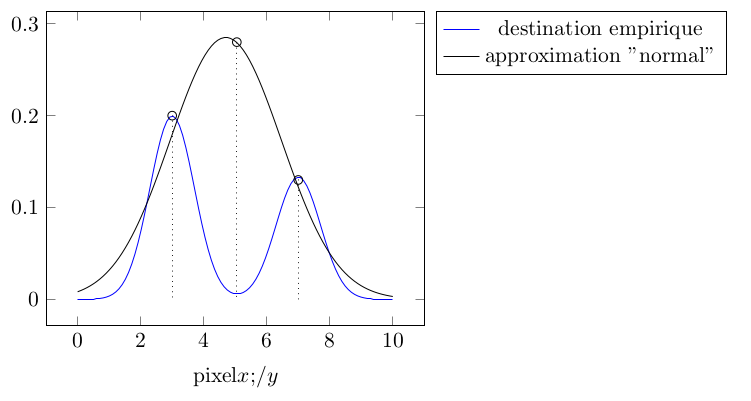
\includegraphics[scale=0.4]{schema4.png}

\begin{itemize}
\item Augmenter la capacité du modèle.
\item Augmenter le nombre de paramètres.
\end{itemize}

\item \textbf{Mélange de Gaussienne (G.M.M.)}

K : Le nombre de Gausiennes / clusters.

\[ P(\vec{x_n} | \Theta) = \sum_{k=1}^k \pi_k N(\vec{u_k}, \Sigma_k) \]

\begin{itemize}

\item Les paramètres $\Theta$ : $(\pi_k, \vec{u_k}, \sum_k)_{k=1}^K$

\item $\pi_k$ est le poids du mélange.

\item $N(\vec{u_k}, \Sigma_k)$ est la loi gaussienne.

\end{itemize}

\end{itemize}

L'objectif de l'apprentissage est d'estimer les paramètres du mélange permettant de :

\begin{itemize}
\item Maximiser $ \Pi_{n=1}^N  P(\vec{X} = \vec{x} | \Theta)$

\item Maximiser $log(\Pi_{n=1}^N P(\vec{X} = \vec{x_n} | \Theta))$ (on retrouve la probabilité vue plus haut).

\end{itemize}

\subsection{Algorithme E.M.}

\begin{itemize}

\item Algorithme itératif qui cherche à maximiser : 

\[ log(P(\vec{X} = \vec{x_n} | \Theta))  \]

\item Introduire des variables \textbf{latentes} (cachées) : 

\begin{itemize}

\item Pour chaque $\vec{x} -> \vec{Z}$ (one-hot vecteur)
\item $\vec{Z} = (0, 0, ..., 1, 0, 0) -> Z_k = 1 <=> \vec{x} \in cluster k$
\item $\vec{Z}$ : 
\begin{itemize}
\item Pseudo-affectation
\item Un vecteur latent
\item Inconnu : $\vec{Z}$ un vecteur aléatoire
\item Affectation "soft" : Un point peut appartenir à tous les clusters.
\end{itemize}
\end{itemize}
\end{itemize}

Résumé du programme : 

Introduction $\vec{Z}$ associé à $\vec{X}$. Si on souhaite maximiser : 
\[ P(X | \Theta) = \sum_Z P(\vec{X}, \vec{Z} | \Theta) \]
\[ P(X | \Theta) = \sum_Z P(\vec{X} | \vec{Z}, \Theta) P(\vec{Z} | \Theta) \]

On note que $P(X | Z, \Theta)$ est la loi normale $N(\vec{u_k}, \Sigma_k)$ et que $P(\vec{Z} | \Theta)$ est $\pi_k$.

Si $\vec{Z_k} = (0, ..., 1, 0) rang k$
\begin{itemize}
\item $(\vec{X}, \vec{Z})$ : Données complètes.
\item $(\vec{X})$ : Données incomplètes.
\end{itemize}

\textbf{Etape E(xpection) : }
\begin{itemize}
\item Connaitre $\vec{Z}$ à $\Theta$ \textbf{fixé}.
\item Calcul la probabilité d'affectation : $P(\vec{Z} |, \vec{X}, \Theta)$
\end{itemize}

\textbf{Etape M(aximization) :} Les données sont incomplètes. On calcule $\Theta$ et on "fixe" $\vec{Z}$.

\subsection{Optimisation variationnelle}

Après l'introduction de $\vec{Z}$, on introduit une distribution auxiliaire sur $\vec{Z}$, notée $q(\vec{Z})$. On souhaite maximiser selon $\Theta$ : 

\[ log(P(X | \Theta) = \sum_{\vec{Z}} q(\vec{Z} log(\frac{P(\vec{X}, \vec{Z} | \Theta)}{q(\vec{Z})} ) - \sum_{\vec{Z}} q(\vec{Z} log(\frac{P(\vec{Z} | \vec{X}, \Theta)}{q(\vec{Z})} ) \]

\[ log(P(X | \Theta)) = log(P(X, Z | \Theta)) - log(P(Z | X, \Theta)) \]

Rappel : $P(X | \Theta) = \frac{P(X, Z | \Theta)}{P(Z | X, \Theta)}$

C'est-à-dire : Le second terme : 

\[ - \sum_{\vec{Z}} q(\vec{Z} log(\frac{P(\vec{Z} | \vec{X}, \Theta)}{q(\vec{Z})} ) = E_{\vec{Z}vq(\vec{Z})} [log(\frac{P(\vec{Z}, \vec{X} | \Theta}{q(\vec{Z})})]  \]

Divergence de Kullback-Leibler (DKL).

\[ DKL(q(\vec{Z}) || P(\vec{Z} | \vec{X}, \Theta)) \]

De chaque côté du "$||$" on a deux distributions sur $\vec{Z}$.

Divergence $\ne$ distance (asymétrique). (faire une phrase...)
\begin{itemize}
\item $DKL(q, P) = 0$ ssi $q = P$
\item $DKL(q, P) \geq 0$ 
\end{itemize}

Le premier terme : $ E_{\vec{Z} v q(\vec{Z})} [log(\frac{P(\vec{Z}, \vec{X} | \Theta}{q(\vec{Z})}))] $ est nommé ELBO (Evidence Lower Bound).

\[ log(P(\vec{X} | \Theta)) = L(\Theta, q) + DKL(q(\vec{Z}) || P(\vec{Z} | \vec{X}, \Theta))  \]

On a $L(\Theta, q)$ une borne inférieure (ELBO). On fait une optimisation par borne inférieure : on maximise la fonction en maximisant sa borne inférieure. Il s'agit d'une maximisation "indirecte".

\textbf{Etape E :} 
\begin{itemize}
\item Les paramètres sont fixés : $\Theta = \Theta^{old}$
\item Maximiser $L(\Theta^{old}, q)$

\[ L(\Theta^{old}, q) = - DKL(q(\vec{Z}), P(\vec{Z} | \vec{X}, \Theta^{old})) + log (P(\vec{X} | \Theta^{old})) \]
\[ q(\vec{Z}) = P(\vec{Z} | \vec{X}, \Theta^{old})  \]

\textbf{Etape M :} Maximiser L selon $\Theta$ avec q fixé.

Illustration :

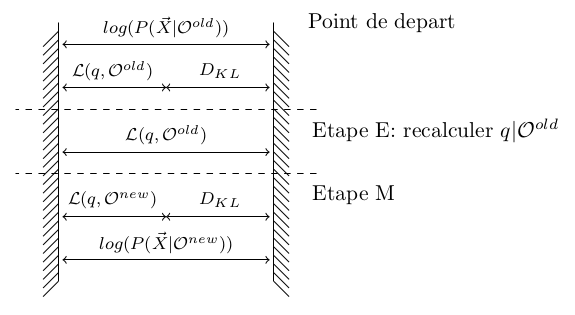
\includegraphics[scale=0.4]{schema5.png}

\end{itemize}

\subsection{Suite du cours}

(A joindre à la subsection algorithme EM ?) \\
\textbf{Remarques :}
\begin{itemize}
\item L'algorithme E.M. est un algorithme d'optimisation.
\item Il augmente notre fonction objectif $P(\vec{X} | \Theta)$ à chaque itération. Si on a un extremum local, on ne va pas maximiser la fonction car on sera bloqué. On ne sortira pas de l'extremum local.
\item De plus, cet algorithme est dépendant des conditions initiales (étape 1 plus bas).
\end{itemize}
\textbf{1.}

\[ log P(\vec{X} = \vec{x} | \Theta) = \sum_Z q(Z = z) log \frac{P(\vec{X} = \vec{x}, Z = z)}{q(Z = z)} - \sum_{Z = z} q(Z) log \frac{P(Z | X}{q(Z)} \]
\[ log P(\vec{X} = \vec{x} | \Theta) = E_{Z \sim q} [ log \frac{P(X, Z)}{q(Z)} - E_{Z \sim q} [log \frac{P(Z | X)}{q(Z)}]  ] \]

\textbf{q} est la distribution auxiliaire. \\
Dans la soustraction : 
\begin{itemize}
\item Premier terme : \textbf{classification sachant Z}. On l'optimise dans l'étape M.
\item Deuxième terme : \textbf{réalisme}. On l'optimise dans l'étape E.
\end{itemize}

\textbf{2. Etape E}

\begin{itemize}

\item Pour chaque $\vec{x}_n$, on calcule sa probabilité d'affectation avec $\Theta$ fixés.

\[ P(Z = k | \vec{X} = \vec{x}_n) = \frac{\pi_k \times N(\vec{u}_k, \sum_k)}{\sum_{k' = 1}^{k} \pi k' \times N(\vec{u}_k', \sum_{k'})  } \]

\item Objectif : $P(Z | \vec{x}; \Theta_{old}) (fleche) q(Z)$

\end{itemize}

\textbf{3. Etape M}

Optimiser un classifieur selon les données qui sont représentées par $q(Z)$ (la fonction auxiliaire). Si on note $a_{nk} = P(Z = k | \vec{x}_n; \Theta_{old})$,
la probabilité d'un cluster :

\[ P(Z = k) = \pi_k = \frac{1}{N} = \sum_n a_{nk} = \frac{N_k}{N} \] 

N est le "nombre d'exemple".

\[ \vec{u}_k = \frac{1}{N} \sum_n a_{nk} \vec{x}_n \]

Qu'est-ce que $a_{nk}$ ? (pas compris)

\[ \sum_k = \sum_n (\vec{x}_n - \vec{\mu}_k) (\vec{x}_n - \vec{\mu}_k) ^{t}  \]

On peut obtenir un nouveau jeu de paramètres $\Theta_{new}$

\textbf{4. Algo E.M.}

\begin{enumerate}
\item Initialisation des paramètres $(\pi_k, \vec{\mu}_k, \sum_k)_{k = 1}^{k}$
\item E : Calcul des "$a_{nk}$" $ | \Theta$
\item M : Calcul de $\Theta | $ "$a_{nk}$"
\end{enumerate}

On boucle entre les étapes 2 et 3 (en général une dizaine de fois) puis l'agorithme se termine.

\end{document}


